%!TEX root = thesis.tex

\chapter{A population of ``clumpy'' galaxies in the local Universe}
\label{chap:5}

Simultaneous to the development of this research was the publishing of the Galaxy Zoo: Hubble galaxy morphology classification catalog. A portion of the original GZ2 SDSS galaxy sample was included in Galaxy Zoo: Hubble because the decision tree for the latter was more complex than that for GZ2. This enabled a comparison between different decision trees and led to the identification of a rare sample of low redshift clumpy galaxies. This chapter details the identification of such a sample, preliminary analysis of the star-forming clumps, and methods to identify more such galaxies in the local universe as these may be analogs of high redshift galaxies with similar properties.


\section{Introduction}
Structural properties of typical galaxies today were forged over the 5 billion years between the peak of cosmic star-formation at $z\sim1.5-2$ and now. Theoretically,  galaxy growth is predominantly governed by the baryonic physics of gas accretion and energy feedback, rather than by mergers that induce starbursts \citep{Somerville2015}. Gas inflow modulates galaxies' star formation histories and plays a crucial role in the dynamical state of the galaxy. A varying gas fraction changes the amount of fragmentation within the gaseous disk, the star-formation rates (SFR), strengths and lifetimes of disk structural components, and possibly the fueling rate of the AGN. As a consequence of the gas accretion process, the small-scale structure within disk galaxies is also predicted to change over time, with the appearance of stable “grand design” spiral arms only at later epochs \citep{Oppenheimer2010,Bouche2010,Dave2011b,Dave2011a,Lilly2013,Hirschmann2013}.

%(e.g. Oppenheimer et al., 2010; Bouch ́ e et al., 2010; Dav ́ e et al., 2011a,b; Lilly et al., 2013; Hirschmann et al., 2013). 

Galaxies along the so-called star-forming main sequence at $z>1.5$ \citep{Noeske2007} tend to be thick, turbulent disks, with specific SFRs of the order of a Gyr, substantially higher than what is observed in the thin, quiescent, Milky-Way-like disks typical of the local universe \citep{Genzel2008}. The SFRs in these ``clumpy'' galaxies is concentrated in a few massive star-forming regions, usually dubbed as star-forming “clumps”, with sizes of approximately $100-1000$pc, stellar masses of $10^7 - 10^9M_{\odot}$, and stellar ages typically younger than the age of the host galaxy \citep[e.g.,][]{Elmegreen2005,Genzel2011, Guo2012,Guo2015}

The origin of these massive clumps is still an open debate. Two main physical scenarios have been proposed. On the one hand, giant clumps are expected to form inside pre-existing galaxies. In these scenarios, halos located at the center of multiple filaments continuously accrete gas from the cosmic web, resulting in the formation of gas-dominated disks that eventually fragment into giant clumps through gravitational instability \citep{Bournaud2007,Dekel2009,Behrendt2015}. Alternatively, clumps may have an external origin, as in the case of mergers with small star-forming companions \citep{Ceverino2010,Bournaud2016}. 

Observationally, the situation is still unclear. Large gas-to-baryonic fractions of 20\% to 80\% recently measured with interferometric studies in clumpy galaxies lends support to the in-situ models \citep{Erb2006,Tacconi2008,Tacconi2010}. Similarly, the kinematics in the majority of these galaxies is characterized by large, regularly-rotating disks, with no signs of on-going or recent mergers \citep{Genzel2006,ForsterSchreiber2009,Epinat2012,Newman2012}. These studies, however, are 1) limited to galaxies with SFR $>10M_{\odot}$ yr$^{-1}$ and $M>10^{10}M_{\odot}$ and 2) include only a few galaxies with high spatial resolution kinematic and interferometric data \citep{Genzel2014}. 

The lack of existing observational constraints below $10^{10}M_{\odot}$ is of particular concern. It is precisely in this mass range that most of the constraining power resides. In fact, state of the art simulations that directly resolve the interstellar medium of individual galaxies while capturing their cosmological environment show that low mass galaxies are mostly affected by preventive feedback \citep{Muratov2015, Christensen2011,Dave2016}. These simulations show that in galaxies with $M<10^{10}$ supernova-driven fast outflows can lower the gas inflow rate and consequently the rate at which clumps are formed in-situ, compared to more massive galaxies. If clumps are the result of minor merging, on the other hand, the dependency with stellar mass would hinge on the specifics of the dynamics of the mergers. 

In this work we utilize the high quality data accumulated by SDSS for a sample of local clumpy galaxies discovered during the preparation of the Galaxy Zoo: Hubble morphology catalog which collected morphological data for galaxies in Stripe 82. Taking advantage of the increased depth of the Stripe 82 coadd imaging for over 100 galaxies, as well as high quality SDSS spectra for more than 150 ``clumps'', we explore the properties of this initial sample to assess how similar these objects are to their high redshift counterparts. Additionally, we seek to differentiate between possible clump formation mechanisms, especially for low mass galaxies of which our sample peaks around $9M_{\odot}$, precisely the range for which observations are sorely needed. In Section \ref{chap5: data} we detail the galaxy selection process and data utilized in this work, followed by a preliminary analysis of various clump properties in Section \ref{chap5: clump properties}. We next discuss the \textit{Clump Scout} project in Section \ref{chap5: Clump Scout}: an initiative to discover up to 1000 more low redshift clumpy galaxies hiding in SDSS imaging data. Finally, in Sections \ref{chap5: future} and \ref{chap5: summary} we present our conclusions and future work. Throughout this chapter we assume a flat Planck cosmology \citep{Planck2016} with H$_0=67.8$ and $\Omega_m = 0.308$ where appropriate. 


\section{Sample Selection \& Data} \label{chap5: data}

We identify a sample of clumpy galaxies in the local universe by considering classifications from both the Galaxy Zoo 2 \citep[GZ2][]{Willett2013} and Galaxy Zoo: Hubble \citep[GZH][]{Willett2017} projects. We provide a brief overview of each of these projects here. 

The GZ2 subject sample consists of 285,962 galaxies identified as the brightest 25\% ($r$-band magnitude $< 17$) residing in the SDSS North Galactic Cap region from Data Release 7 and included subjects with both spectroscopic and photometric redshifts out to $z < 0.25$. In addition to the DR7 Legacy catalog, galaxies were included from Stripe 82, a multiply-imaged strip along the celestial equator in the Southern Galactic Cap. Galaxies in this region were selected to have $m_r\le17.7$ and petror90\_r $>3$, where petror90\_r is the radius containing 90\% of the r-band Petrosian aperture flux.


%OK -- and so what? you leave the reader hanging... all of this is good but what is the solution? Fuck if I know, bitch.


\begin{figure}
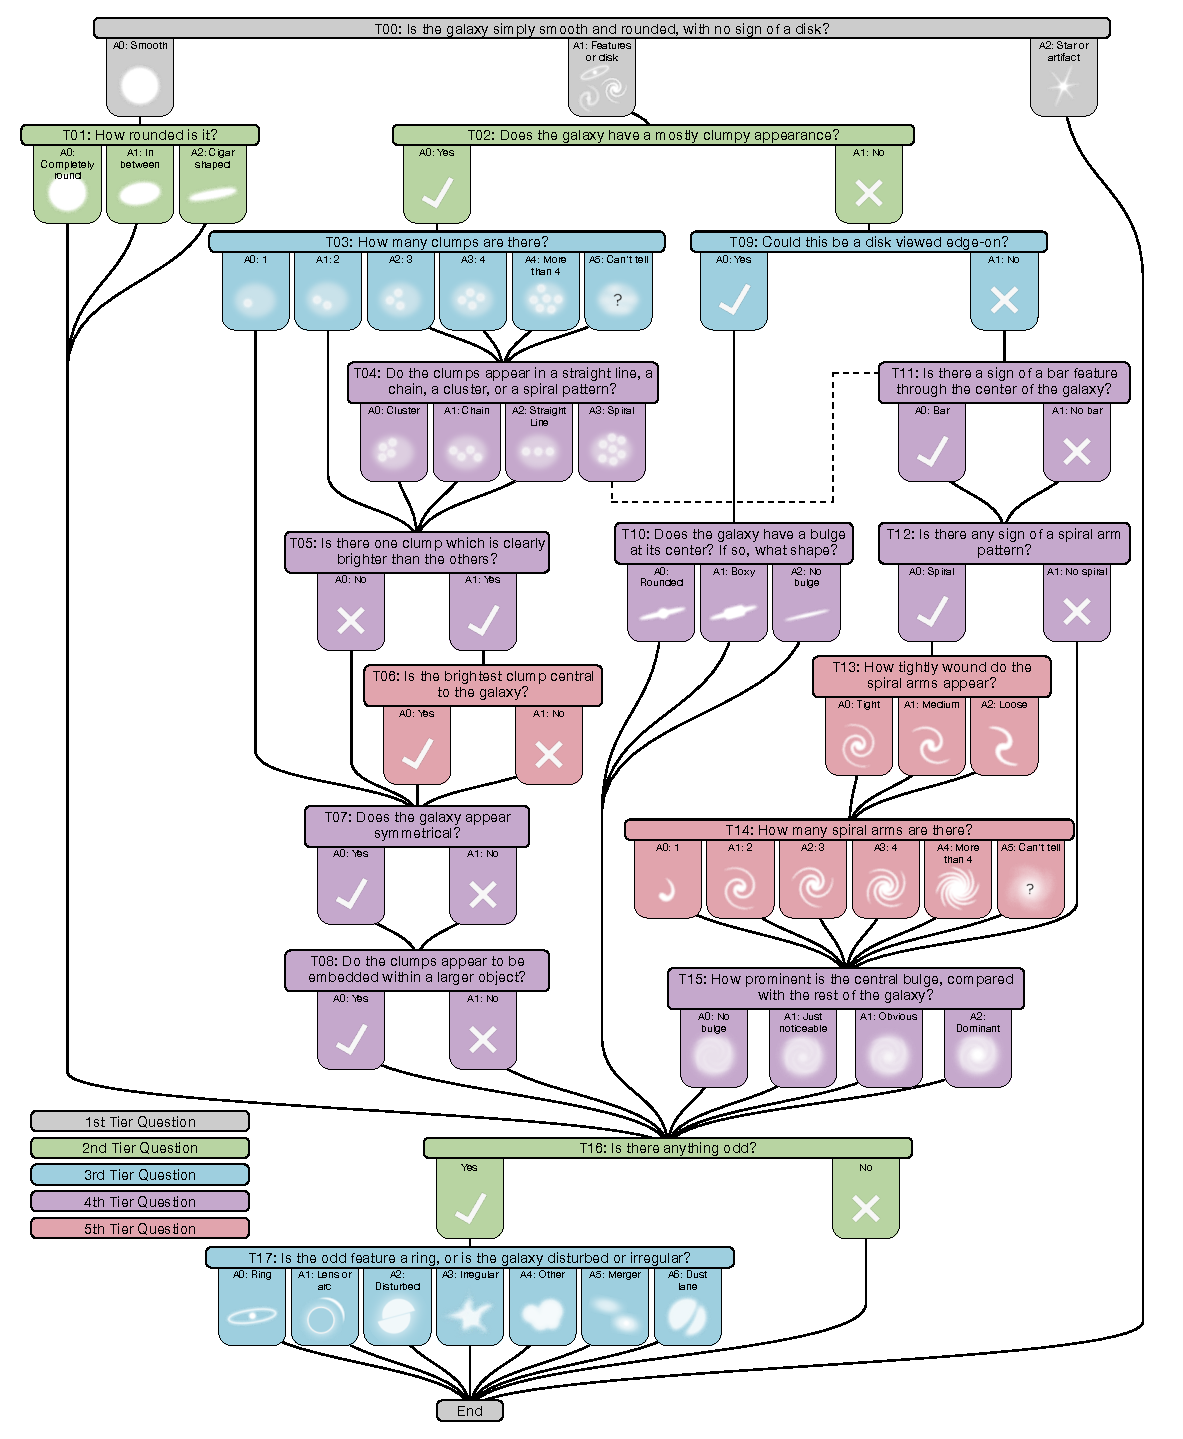
\includegraphics[width=\textwidth]{Figures/gz3_tree_resized.pdf}
\caption[Galaxy Zoo: Hubble decision tree.]{Galaxy Zoo: Hubble decision tree. The most notable difference between this decision tree and that used during the Galaxy Zoo 2 project is the ``clumpy'' branch of tasks.}
\label{fig: gzh decision tree}
\end{figure}

The GZH project contains images drawn from several dedicated surveys and sample selection criteria. Most samples are drawn from various Hubble fields such as AEGIS, GOODS and COSMOS; however also included are the single-epoch and co-added images from Stripe 82 of the SDSS Data Release 7 that were part of the GZ2 project. The single-epoch imaging allows for local comparison to higher redshift galaxies, while the co-added imaging allows for image depth analyses. 

The most notable difference between these two projects is the decision tree presented to volunteers. The goal of GZH was to collect detailed morphologies for galaxies in Hubble imaging which extends to much higher redshift than those of the SDSS sample. Galaxies at higher redshift do not necessarily follow the traditional Hubble sequence and thus a new branch of questioning was added to the decision tree for this project, shown in Figure \ref{fig: gzh decision tree}. This included several questions concerning the clumpy nature of galaxies, a morphological feature well known to exist at higher redshift. Because GZH included galaxies from the GZ2 project, we can draw on both sets of decision trees to identify clumpy features for galaxies in Stripe 82.


To select a sample of ``clumpy" galaxies from the GZH Stripe 82 sample, we consider only those subjects with large featured (\ffeat) and clumpy (\fclump) vote fractions: the fraction of volunteers who voted a subject as `featured or disk' in response to the first question ``Is the galaxy simply smooth and rounded, with no sign of a disk?'' and who answered `yes' to the question ``Does the galaxy have a mostly clumpy appearance?'' Specifically, we select galaxies which satisfy \ffeat~$\ge0.5$ and \fclump~$\ge0.5$ Additionally, we require $N_{\mathrm{votes}} \ge 20$, where $N_{\mathrm{votes}}$ is the number of volunteers who answered the clumpy question. This insures that \fclump~is statistically significant and not a product of too few votes.  This yields a sample of 629 galaxies: 273 single-epoch imaging and 356 from the co-added imaging. After visual inspection we find that this is hardly a pure sample of clumpy galaxies in the traditional sense, instead including a sizable sample of tight groups of elliptical galaxies, as well as galaxies in various merging states, possessing multiple nuclei. After excluding these and duplicate imaging, we retain 92 coadd-depth and 105 single-depth clumpy galaxies, of which 156 are unique systems (some objects are common to both the single-epoch and coadd-depth imaging). Finally, we exclude galaxies with $z>0.06$ in order to retain a sample wherein the physical scale as observed by SDSS is similar to Hubble's at $z\sim3$ to allow for comparison with high redshift samples. Our final sample contains 104 unique galaxies. SDSS \textit{gri} color-composite jpegs for all galaxies can be found at the end of this work in Section \ref{chap5: jpegs} where SDSS's spectroscopy flag is enabled, generating a red square around each spectroscopic target.  

\begin{figure}
\centering
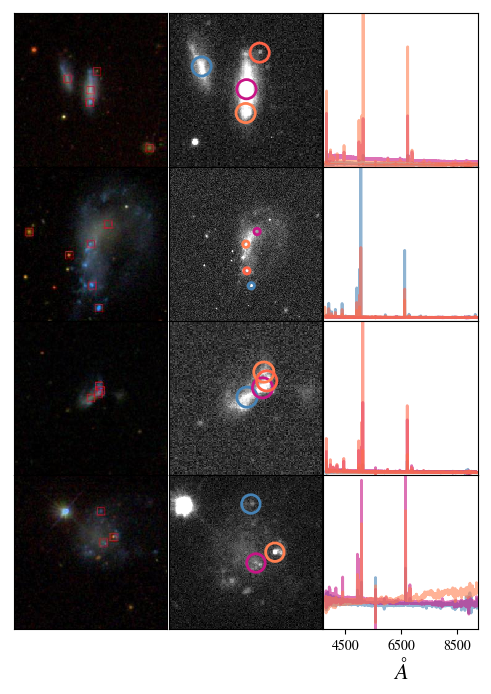
\includegraphics[width=4.75in]{Figures/jpeg_fits_spec_examples.png}
\caption[Sample of ``clumpy'' galaxies determined by Galaxy Zoo: Hubble]{Sample of ``clumpy'' galaxies. The first column shows the SDSS $gri$ color composite image where the red squares denote locations of SDSS spectroscopy. The middle column shows our postage stamp for the object where the colored circles show the same spectral locations, however these circles are color coded to the third panel which shows the spectra associated with each object.}
\label{fig: clumpy examples}
\end{figure}


We obtain SDSS Data Release 12 (DR12) \textit{ugriz} coadd imaging, as well as all optical spectra associated with each galaxy. The wavelength range of the SDSS spectra is $3800-9200$\AA~with a resolution of $R\sim 1500$ at $\sim3800$\AA. The $3$\arcsec~SDSS fibers cover 2.9 kpc at $z=0.05$. We visually inspect all spectra to verify that they are associated with an object in our sample as opposed to a nearby object or overlapping star. Through this inspection we determine that one clumpy galaxy is actually a juxtaposition of three galaxies at disparate redshifts flagged as clumpy in GZH due to the low resolution of SDSS imaging. We exclude this subject from our sample. Our final list includes 171 spectra. Approximately half of the galaxies in our sample have more than one spectrum with a handful having three or four spectra. Figure \ref{fig: clumpy examples} shows some examples of our clumpy galaxies where the first column is the $gri$ color composite SDSS jpeg image with red squares denoting the location of SDSS spectra. The middle column shows the $r$-band postage stamp (described below) where the colored circles again denote the location of SDSS spectra and reflect the size of the fiber. The third column shows the spectra associated with each object, color-coded to the apertures in the middle column. 


We create postage stamps of each galaxy from the $r$-band SDSS fields.  The size of the postage stamp is taken to be 3$\times\mathtt{petrorad\_r}$, the Petrosian radius as measured in the $r$-band by the SDSS pipeline. We then run Source Extractor \citep{sextractor} on each postage stamp. During visual inspection of these cutouts and the associated SExtractor segmentation maps we discover that the SDSS coordinates are occasionally incorrectly assigned, that is, star-forming clumps are mistaken for individual galaxies likely due to the low surface brightness of some of these systems. An example is shown in the final row of Figure \ref{fig: clumpy examples}. It is clear in the first panel that the central coordinates are not well aligned with the galactic center. The middle panel depicts our postage stamp in which we have corrected the galaxy's coordinates using that determined by SExtractor. 

\begin{figure}
\centering
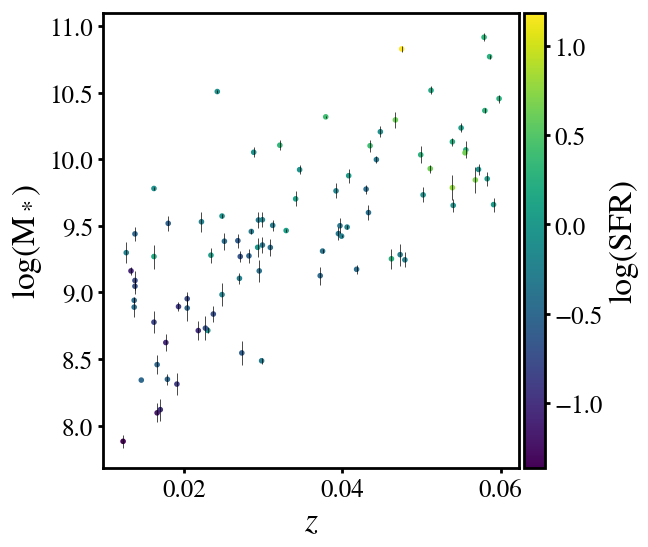
\includegraphics[width=5in]{Figures/mass_z_sfr.png}
\caption[Stellar mass, redshift, and Star-formation rate for a subset of our ``clumpy'' galaxies as measured by the GSWLC.]{Stellar mass, redshift, and star-formation rate (SFR) for a subset of 89 ``clumpy'' galaxies as estimated by \cite{Salim2016} in the GSWLC. With a median log $M_{\odot}=9.4$, our sample includes dozens of low mass galaxies that will be crucial for helping to constrain models of star-formation in low mass galaxies.}
\label{fig: clumpy gswlc properties}
\end{figure}


We also draw on the \textit{GALEX}-SDSS-\textit{WISE} Legacy Catalog \citep[GSWLC,][]{Salim2016} which provides stellar mass, star formation rates (SFR) and dust attenuations for 700,000 low-redshift galaxies. Specifically we obtain the GSWLC-X version which contains measurements using the deepest imaging available for each galaxy in the sample. We provide a brief overview of their methodology here.  Galaxy physical properties were obtained from UV and optical spectral energy distribution (SED) fitting utilizing imaging data from the \textit{Galaxy Evolution Explorer}, SDSS, and \textit{Wide-field Infrared Survey Explorer} surveys for galaxies with $z<0.3$, covering up to 90\% of the SDSS footprint. \cite{Salim2016} use a Bayesian fitting methodology that includes corrections for photometry blending and emission-lines.  We match our sample against this catalog to objects within $15\arcsec$, of which we find 95. Of these, 6 are flagged as having failed the SED fitting and are thus excluded. Thus we retain 89 galaxies with estimates of global galactic parameters. Figure \ref{fig: clumpy gswlc properties} shows the distribution of our sample wherein we plot the galaxy log stellar mass as a function of redshift with color denoting the log SFR. The median galaxy log stellar mass for our sample is $\sim9.4 M_{\odot}$. 


%The physical scale at z= 0.06 is 1"=1.1kpc. SDSS pixel scale is 0.396"/pixel. --> 0.43 kpc/pixel -->  ~2.3 pixels = 1kpc.  We visually inspect these spectra and verify that the fiber was positioned over a star-forming region in the majority of cases rather than the galactic bulge or other structure. 



\section{Are these star-forming regions analogs of high-redshift clumps?}
\label{chap5: clump properties}

Several studies have been conducted which examine the properties of both local HII regions and high-redshift star-forming clumps \citep[e.g.,][]{Monreal-Ibero2007,Swinbank2009,Wisnioski2012} but the debate between whether these regions arise due to the same physical processes remains unresolved. That these regions arise through different physical mechanisms would not be surprising given the stark changes in the global environments of galaxies between those at Cosmic Noon and of today. In particular, gas accretion rates which drive up turbulence and sustain disk instabilities are expected to dissipate on cosmic timescales, at least for massive galaxies \citep{Dekel2006}. However, \cite{Wisnioski2012} show that despite these changes, similarities between local HII regions and clumps at $z\sim1.3$ persist in the form of several elegant scaling relations. In this section we revisit some of these relations with the goal of ascertaining whether the star forming regions in our sample could pose as analogs of high redshift clumps. 

Specifically, we exploit the high quality emission line measurements produced through the SDSS spectroscopic pipeline. Most of these fibers are either centered on a bright star-forming region which we interpret as a ``clump,'' or on/near the galactic center (see Section \ref{chap5: jpegs} for reference). If clump lifetimes are longer than the dynamical time of the galaxy it is possible that they migrate to the galactic center, contributing to bulge formation. We thus do not remove those spectra that are close to the central regions of their host galaxy so as not to bias ourselves against this possibility. 

\subsection{H$_{\alpha}$ luminosity and velocity dispersion}
\label{chap5: luminosity}

\cite{Wisnioski2012} develop empirical scaling relations between clump size, luminosity, and velocity dispersion for a sample of local HII regions along with a sample of high redshift clumps. They demonstrate that these relations hold over three orders of magnitude in clump diameter and five orders of magnitude in \ha~luminosity for thousands of local HII regions and high-redshift clumps taken from 11 different studies. We briefly describe two of these relations here. 


\begin{figure}
\centering
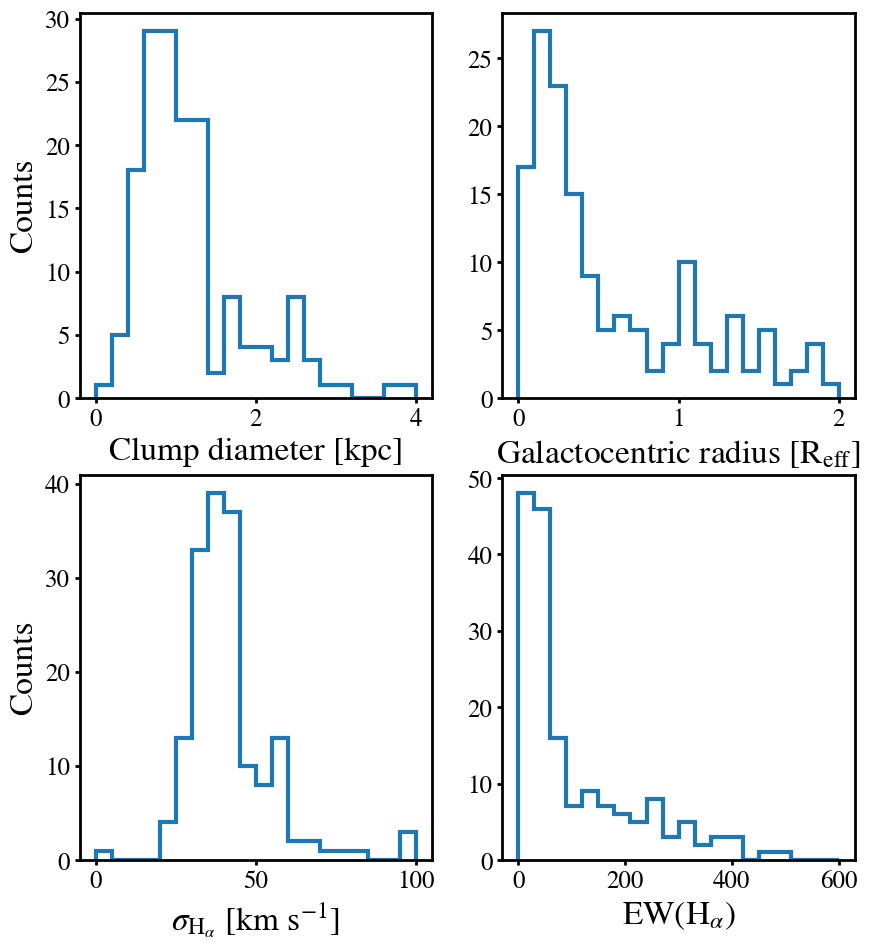
\includegraphics[width=5in]{Figures/clump_4properties.png}
\caption[Histogram distributions of several physical properties for $\sim$170 ``clumps.'']{Distributions of several physical properties of the $\sim$170 star-forming regions in our sample. These properties (with the exception of galactocentric radius, see Section \ref{chap5: galactocentric radius}) are all derived from emission-line measurements produced by the SDSS spectroscopic pipeline. }
\label{fig: clump histograms}
\end{figure}

If a star-forming region can be idealized as a Str{\"o}mgren sphere of radius, r, then it is straightforward that a scaling relation between \ha~luminosity and the size of the region should exist. A Str{\"o}mgren sphere describes the region of ionized HII surrounding hot, young O-B stars and the \ha~luminosity of such a region scales as $r^3$, where this radius is assumed to be the clump radius. Under this assumption, \citep{Wisnioski2012} fit the following relation:

\begin{equation}\label{eqn: luminsotiy-size}
\log(L_{\mathrm{H}_{\alpha}}\ [\mathrm{erg s}^{-1}]) = 2.72\times\log(\mathrm{d\ [pc]})+31.99
\end{equation}
where $d$ is the clump diameter in units of pc. 

They derive a similar relation between velocity dispersion and size under the assumption that these regions form out of a Jeans collapse in an isothermal disk. Under this scenario, the clump radius is assumed to correspond to $\lambda_{\mathrm{J}}/2$, where $\lambda_{\mathrm{J}}$ is the Jeans length which scales with velocity dispersion as $\sigma^2$. With this assumption, \cite{Wisnioski2012} determine a velocity dispersion-size relation according to

\begin{equation}\label{eqn: sigma-size}
\log(\sigma\ [\mathrm{km\ s}^{-1}]) = 0.42\times\log(\mathrm{d\ [pc]})+0.33
\end{equation}
where again $d$ is the clump diameter in units of pc.

We begin by estimating the \ha~flux and velocity dispersion for each spectrum as measured by a Gaussian fit to the emission line in the SDSS spectroscopic pipeline. Additionally we correct the \ha~velocity dispersion by subtracting in quadrature the SDSS instrument resolution. In this preliminary analysis we do not correct the \ha~flux for dust attenuation. In the bottom left panel of Figure \ref{fig: clump histograms} we show the distribution of the \ha~velocity dispersion for all spectra in our sample, where the median is $\sigma_{\mathrm{H}_{\alpha}}\sim40$km/s. While this is slightly smaller than giant star-forming regions observed at $z\sim$2 \citep{Elmegreen2010,Sanchez2013}, it is also significantly larger than typical HII regions observed in local galaxies. From this, we estimate the clump diameter according to equation \ref{eqn: sigma-size}. The resulting clump diameter distribution is shown in the top left panel of Figure \ref{fig: clump histograms}. The median diameter is $\sim$1 kpc which is larger than the average local HII region but slightly smaller than high redshift clumps.  Keep in mind that some of these ``clumps'' could actually be the central bulge region of some systems since we do not specifically separate them as discussed earlier. The central regions will typically have much lower rates of star formation, smaller \ha~velocity dispersion, and thus significantly smaller sizes according to this relation. If these regions were excluded, the median diameter would be more typical of high-redshift clumps. In a more detailed analysis, clump sizes will be confirmed independently through a ``core'' analysis whereby sizes are measured by fitting a Gaussian to the 1D radial surface brightness profile of each star-forming region.  

The left panel of Figure \ref{fig: clump scatter plots} shows the relationship between the \ha~luminosity and the clump diameters derived from the \ha~velocity dispersion. The black dashed line represents the luminosity-size scaling relation of equation \ref{eqn: luminsotiy-size}. The points are color-coded according to the stellar mass of the host galaxy and the black squares are those spectra whose corresponding galaxy does not have a match in the GSWLC. The clumps in our sample lie reasonably well along the empirical relation of \cite{Wisnioski2012} though much of the sample has lower \ha~luminosity. The \ha~luminosity distribution overlaps with that of high redshift clumps, though the size distribution is intermediate between local and high-redshift star-forming regions, as previously discussed. There is also a strong galaxy stellar mass dependence along the relation. This isn't altogether surprising since lower mass galaxies typically have smaller SFRs in our sample (as evidenced by the global SED SFR in Figure \ref{fig: clumpy gswlc properties}) and, by extension, lower \ha~luminosities. 

\begin{figure}
\centering
\includegraphics[width=\textwidth]{Figures/Wisnioski_HaLum_vs_clumpDiameter.png}
\caption[Clump properties: $L(\mathrm{H}_{\alpha})$ vs size and $\sigma_{H_{\alpha}}$ vs $\Sigma_{SFR}$]{In the left panel we show the \ha~luminosity versus clump size as estimated via the \ha~velocity dispersion utilizing equation \ref{eqn: sigma-size}. The black dashed line represents the luminosity-size relation of \cite{Wisnioski2012}, reproduced in equation \ref{eqn: luminsotiy-size}. The right panel shows the \ha~velocity dispersion versus the clump star formation rate density. In both panels the points are colored according to host galaxy total stellar mass as measured by \cite{Salim2016} in the GSWLC. The black squares are those clump spectra whose host galaxy did not match to that catalog.}
\label{fig: clump scatter plots}
\end{figure}

Several observations have detected a relationship between luminosity and velocity dispersion of galaxies both locally and at high redshift \citep{Dib2006,Green2010,Lehnert2009,Genzel2011}. It has been suggested that the velocity dispersion is driven by star formation. One possibility is through released mechanical energy as discussed in \cite{Lehnert2009}. \cite{Wisnioski2012} offer an alternative whereby the velocity dispersion is the result of the star formation density in a marginally stable galactic disk (i.e., Toomre parameter, $Q\sim1$), assuming the Kennicutt-Schmidt law, an empirical relation between SFR surface density ($\Sigma_{\mathrm{SFR}}$) and gas surface density \citep{Schmidt1959,Kennicutt1998a}. While \cite{Wisnioski2012} find a moderate correlation between $\sigma-\Sigma_{\mathrm{SFR}}$, \cite{Genzel2011} find a weak dependence concluding that feedback does not appear to directly drive the velocity dispersion of the ionized gas.  Utilizing the clump sizes measured previously, we estimate the $\Sigma_{\mathrm{SFR}}$ after computing the \ha~SFR using the well known calibration \citep{Kennicutt1998,Calzetti2013}
\begin{equation}
\mathrm{SFR} (\mathrm{M}_{\odot} \mathrm{yr}^{-1}) = 5.5 \times 10^{-42}L(\mathrm{H}_{\alpha}) (\mathrm{ergs\ s}^{-1})
\end{equation}
The right panel of Figure \ref{fig: clump scatter plots} shows the resulting $\sigma_{\mathrm{H}_{\alpha}}-\Sigma_{\mathrm{SFR}}$ relation, where again the points are colored according to the host galaxy stellar mass as given by the GSWLC with purple points denoting those spectra for which the host galaxy is not found in that catalog. Instead, we observe a mild anti-correlation. If this finding holds, it could be an indication that feedback mechanisms in low mass galaxies are poorly understood since our sample probes much lower galaxy stellar mass and it is precisely this population that skews the relation. 


Finally, we compare SFRs between those derived from the \ha~emission and the global SED SFR from the GSWLC. For each galaxy, we sum the SFR$_{\mathrm{H}_{\alpha}}$ from each spectrum and compare that to SFR$_{\mathrm{SED}}$, for those 89 galaxies that were matched to the GSWLC. The median ratio of these two star-formation measures is $\sim$10\%. Because a majority of galaxies have only one spectrum, we interpret this rough estimate as being not dissimilar to giant star-forming regions found at high redshift where it is typical for individual clumps to contribute 10\% or more to the total star formation of the galaxy \citep{Genzel2011, Guo2012, Wisnioski2012}.


\section{Physical properties vs galactocentric radius}
\label{chap5: galactocentric radius}

Two broad scenarios for giant clump formation make distinct predictions for the distribution of clump physical properties. If most clumps have an ex-situ origin then there should exist a random distribution of clump properties \citep{Bournaud2008,WuFoSch2012}. On the other hand, most in-situ models suggest that clumps tend to be long-lived (few hundreds Myrs) and migrate to the galaxy center where they coalesce to form a bulge \citep{Bournaud2016}. An age gradient is therefore expected with older clumps preferentially located closer to the galactic center. In this section we search for other possible trends with galactocentric radius though in Section \ref{chap5: future} we discuss the next phase of this project which is to measure the metallicity and stellar ages of these clumps to further constrain clump formation theories. 


We compute the galactocentric distance of each SDSS fiber from the galaxy center as measured by SExtractor, rather than the coordinates provided by SDSS since it was found  that some of these coordinates were centered improperly, as discussed in Section \ref{chap5: data}. We compute the galactocentric distance both in kpc and normalized by the galaxy's half light radius (\texttt{FLUX\_RADIUS}) as determined by SExtractor. The resulting distribution is shown in the top right panel of Figure \ref{fig: clump histograms}. That the distribution is obviously skewed towards the small galactocentric values is likely due to the several spectra that probe the central region. In Figure \ref{fig: galactocentric radius relations} we show several physical properties of clumps as a function of galactocentric radius where the color scheme is the same as described in the previous section. Though no strong trends are seen, some curious insights can still be gleaned.
  

\begin{figure}
\includegraphics[width=\textwidth]{Figures/clump_galactocentric_kpc.png}
\caption[\ha~EW, SFR, Balmer decrement as a function of clump galactocentric radius.]{\ha~equivalent width, star formation rate, and Balmer decrement as a function of clump galactocentric radius normalized by the host galaxy's R$_{\mathrm{eff}}$. In all panels the points are colored according to host galaxy total stellar mass as measured by \cite{Salim2016} in the GSWLC. The dark purple points are those clump spectra whose host galaxy did not match to that catalog.}
\label{fig: galactocentric radius relations}
\end{figure}


 The first panel of Figure \ref{fig: galactocentric radius relations} shows the restframe \ha~equivalent width versus galactocentric radius (the distribution of all EW(\ha) for our sample is shown in Figure \ref{fig: clump histograms}). This is a rough stand-in for specific SFR since it is the ratio of a strong star formation indicator (\ha~line flux) and a reasonable proxy for stellar mass, i.e., the stellar continuum at \ha~\citep{MarmolQueralto2016}. We find that clumps with the strongest EW are more likely to be closer to the galactic center and that clumps far from the center are dominated by low EW. That we find few examples of high EW regions at large radius is interesting as SDSS should be sensitive to this region of the parameter space. In the middle panel we show the relation between the \ha~SFR and galactocentric radius wherein we find that, at large radius, clumps are slightly more likely to have high SFRs. Similar results are found by  \cite{Soto2017} where that trend was accompanied by a trend of young clump ages preferentially located at greater galactocentric radius. Such a scenario is consistent with clump migration theories. There also exists a mild trend with global galaxy stellar mass but this is expected as clump SFRs correlate with the global property as previously discussed. In the final panel, we show the Balmer decrement (\ha/H$_{\beta}$), which probes dust attenuation.  We find that the highest levels of attenuation are found in regions located closest to the galactic center but that significant levels are found in clumps located at large radii.  Furthermore there is a mild galaxy stellar mass dependence wherein lower mass galaxies typically have regions with lower Balmer decrement. 



\begin{figure}
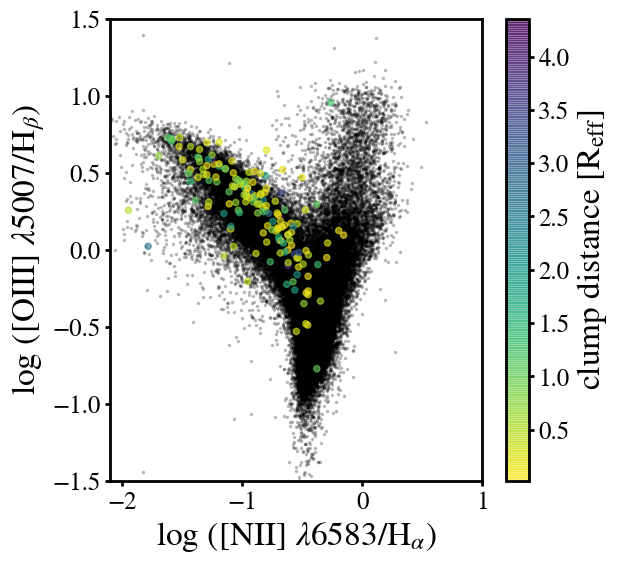
\includegraphics[width=\textwidth]{Figures/bpt2.png}
\caption[BPT diagram of spectra in this sample compared to all SDSS spectroscopic targets.]{BPT diagram of the spectra in our sample color-coded according to clump galactocentric radius against all SDSS spectroscopic targets (black). The red and blue dashed lines represent the theoretical cutoff for star-forming and composite galaxies as determined by \citep{Kewley2006}. As expected, the majority of the regions in our sample are well situated on the star-forming branch of the diagram though there does not appear to be any relation with galactocentric distance.}
\label{fig: bpt}
\end{figure}

Finally, we compare our sample with the full SDSS Data Release 8 spectroscopic catalog (black) on the BPT diagram in Figure \ref{fig: bpt}. The BPT diagram utilizes a set of nebular emission lines to distinguish between various ionization mechanisms of nebular gas \citep{Baldwin1981}. Though several versions exist, we use the most common \oiii/\hb~versus \nii/\ha. As both ratios are based on lines close in wavelength, effects due to reddening are negligible. Here our regions are colored according to galactocentric radius. The red and blue dashed lines represent the theoretical cutoff for star-forming and composite galaxies as determined by \citep{Kewley2006}. As expected, the majority of our clumps lie comfortably in the star-forming region of the BPT diagram though a handful of spectra fall in the composite region (between the red and blue dashed lines), and one spectrum lies well within the AGN range in the upper right-hand portion of the diagram. In the future we will follow up on these few outliers to determine their true identity. There does not appear to be a correlation of the ionization states of these spectra with clump galactocentric radius. This is not necessarily surprising since, to our knowledge, no trend on clump specific ionization state has been predicted. 


%Considering galaxies of a few $10^{10}$ Mstar, a small companion of about $10^9$ Mstar should be found within a projected distance of 10kpc for about 1/3 of galaxies Bournaud2016 based on the mass fucntion of galaxies and assuming a random geometrical distribution of satellites within the virial radius. If the satellite is not disrupted by the galactic tides, its nucleus should be observed as a giant clump. Ex-situ clumps with older average stellar ages  ... might also be dustier? redder? less ionized? 



%=========================================================================
%	CLUMP SCOUT
%=========================================================================
\section{Clump Scout}
\label{chap5: Clump Scout}

The above analysis was performed on a subsample of galaxies determined as ``clumpy'' from the SDSS Stripe 82 sample included in the GZH project. However, the area covered by Stripe 82 was only a fraction of the full SDSS sky coverage. In this section we describe the \textit{Clump Scout} project, a citizen-science initiative to discover more ``clumpy'' galaxies in the remaining SDSS footprint. We begin with the remaining non-Stripe 82 SDSS galaxies that were originally part of the GZ2 project. We exclude any galaxies with $z>0.06$ in order to satisfy the resolution requirements discussed above. We also make a cut such that \fsmooth~$\le0.8$ in order to exclude those galaxies which are obviously elliptical and would likely not have traveled down the clumpy track of the GZH decision tree. These criteria yield a sample of $\sim63$K galaxies as shown in Figure \ref{fig: clump scout sample} where we depict galaxy number density contours in the $z$-\fsmooth~plane. The red dashed lines denotes the \textit{Clump Scout} sample region. Based on the statistics of the clumpy galaxies found in the sky area of Stripe 82, we expect to find approximately 1000 such systems in the non-Stripe 82 SDSS sky coverage.

The goal of the project is to collect additional volunteer morphology information on par with that collected for the Stripe 82 sample in GZH. We will display jpeg images to volunteers via the Zooniverse Project Builder web platform which also hosts the Galaxy Zoo project.  However, because we have such a large galaxy sample to go through, we will ask volunteers a slightly modified version of the top level question of the clumpy branch of the GZH decision tree in order to increase the speed of classification. Specifically, we ask one question, "Does the galaxy have a mostly clumpy appearance? If so, use the Clump Clicker tool to click the clumps you see." This takes advantage of the Zooniverse Point Tool which marks the location on the image with each click a volunteer makes. This will provide an affirmation of a clumpy galaxy, a preliminary clump count, and coarse clump localization information. We have already created a pilot version of this project which consisted of 1000 galaxy images in two different ``zoom'' levels and received favorable reviews from volunteers who participated. 

\begin{figure}
\centering
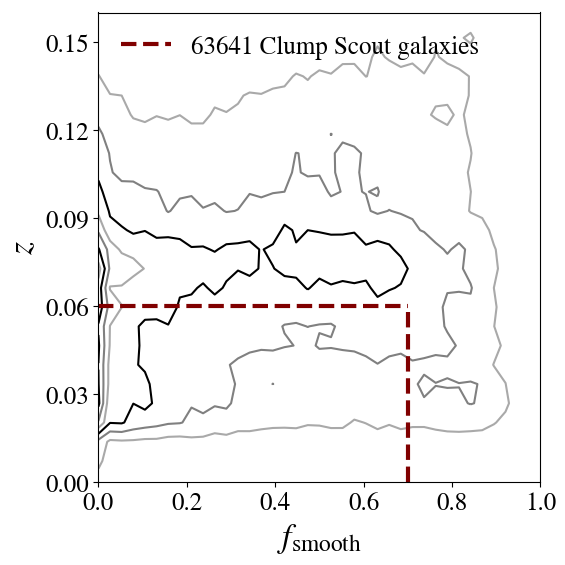
\includegraphics[width=5in]{Figures/clump_scout_sample_in_z-fsmooth.png}
\caption[\textit{Clump Scout} sample selection criteria from non-Stripe 82 GZ2 galaxy sample.]{\textit{Clump Scout} sample selection criteria from non-Stripe 82 GZ2 galaxy sample.}
\label{fig: clump scout sample}
\end{figure}



%In order to secure reliable measurements for \fclump~in the local universe, we must estimate the completeness of recovering low redshift clumpy galaxies from the SDSS sample. Ideally, we  To that end we need to conjure up some simulated clumpy galaxies that span the galactic mass and clump mass range appropriate for XXX reasons. 


\section{Future work}
\label{chap5: future}

The analysis presented thus far is unable to constrain clump formation models. In this section we detail the next phase of this work for which we recently received an NSF grant. 
The in-situ and ex-situ models for giant clump formation make distinct predictions for the distribution of the clumps’ metallicities and stellar ages. If clumps really formed within their host galaxy, statistically some newly formed ones (age $< 20$ Myr) should be observed within the preexisting galactic disk. Also, the metallicity of the gas associated with the youngest clumps should be similar to the metallicity of the gas surrounding the clumps. Conversely, if the observed giant clumps are of external origin, they would be expected to show a broad range of stellar ages and metallicities, and often large deviations from the host disk velocity field \citep{Bournaud2008,WuFoSch2012}. Additionally, these properties are expected to vary with the galactocentric radius because in in-situ models, clumps tend to be long-lived (few hundreds Myrs) and migrate to the galaxy center where they coalesce to form a bulge \citep{Bournaud2016}. An age gradient is therefore expected, with older clumps being preferentially located closer to the galaxy center. Recently, however, this paradigm has been questioned as simulations incorporating more realistic feedback find that clumps are not long-lived \citep{Genel2012,Hopkins2012,Oklopcic2017}. Although some observational constraints do exist, they are mostly based on studies of broad band images, and very limited spectroscopic data are available \citep{Guo2012,Zanella2015}. 

The quality of the SDSS spectra will allow us to derive accurate stellar ages (from fitting of the continuum) as well as gas metallicity \citep{Henry2015}. By combining our current sample with those discovered through the \textit{Clump Scout} project, we will be able to derive statistical trends in the clumps properties. We will group the clump properties according to galaxy stellar mass, distance from the galaxy center, and environmental density. 


\begin{figure}
\centering
\includegraphics[width=3in]{Figures/guo15.png}
\caption{Adapted from \cite{Guo2015} to emphasize how in the $0 - 1$ redshift range (approximately half the age of the universe), observations of the fraction of clumpy galaxies are still highly unconstraining.}
\label{fig: clumpy fraction}
\end{figure}


Additionally, this large statistical sample will allow us to investigate the evolution of the fraction of clumpy galaxies as a function of cosmic time, \fclump~(not to be confused with the GZH clumpy vote fraction). \cite{Guo2015} recently showed that the fraction of star-forming galaxies that have at least one off-center clump (\fclump) can be used to place constraints on theoretical models. By focusing on the redshift range between $0.5 <z<3$, they find that \fclump~changes with the stellar mass of the galaxies. Low-mass (log M $<10$ M$_{\odot}$) galaxies keep an almost constant \fclump~of $\sim$60\% from $z\sim3$ to $z\sim0.5$, while massive galaxies drop their \fclump~from 55\% at $z\sim3$ to 15\%, at $z\sim0.5$. \cite{Guo2015} argue that these observations support a model in which the clumpy star-formation results from multiple processes. In massive galaxies, the evolutionary trends are consistent with violent disk instability, however the apparent lack of \fclump~evolution in low mass galaxies is more consistent with a minor merger origin. However, this conclusion is based primarily on the lowest redshift bin probed by the \cite{Guo2015} data. In fact, when these data are combined with \fclump~measured from a variety of different surveys at $z<1$, the result is not so convincing anymore, as shown in Figure \ref{fig: clumpy fraction}, adapted from \cite{Guo2015}. The variation in the low-z measurements quite large and is primarily a consequence of non-uniform selection criteria and uncontrolled-for biases. \textit{Clump Scout} promises to provide the largest sample to date selected in a uniform fashion and with biases properly accounted for, especially in the low-mass regime where measurements of \fclump~can provide the strongest model constraints.



\section{Summary and conclusions}\label{chap5: summary}

In this work, we have isolated a sample of galaxies with morphologies which resemble those of star-forming clumpy galaxies of the high-redshift universe. We identify these galaxies in the local universe through the Galaxy Zoo: Hubble project which included imaging from Stripe 82 of the SDSS. We isolate 104 galaxies that have a traditional clumpy morphology and acquire SDSS imaging and spectroscopic data for these galaxies, including spectra for over 150 clumps. These galaxies have a median log stellar mass of 9.4, a sample that could provide crucial constraints on star formation models of low mass galaxies. We obtain stellar mass and star-formation rates for these galaxies through the GSWLC catalog. Our preliminary analysis of the spectra reveals that star-forming regions in these galaxies are in many ways similar to high-redshift clumps: our clumps have a median physical size of $\sim1$kpc and median \ha~velocity dispersion of $\sim40$km/s, values that are only slightly lower than high redshift clumps. We also compare several spectroscopically derived properties with clump galactocentric radius but find no strong correlations. 

These findings motivate not only a more in depth analysis of this sample but also justify the search for similar galaxies in the local universe. To that end we described the \textit{Clump Scout} project designed to search for additional clumpy galaxies in the local universe by presenting color-composite SDSS non-Stripe 82 imaging to the general public. We have made preliminary tests of this project with highly favorable reviews from volunteers and expect to find an additional 1000 clumpy galaxies, with upwards of $\sim1500$ associated spectra. This will provide a large statistical sample of local clumpy galaxies which we will use to constrain the fraction of clumpy galaxies at low redshift, as well as investigate the age and metallicity of individual clumps as a function of galaxy stellar mass, galactocentric distance, and environmental density, allowing us to distinguish between various clump formation theories.  


\section{Visual catalog of SDSS Stripe 82 clumpy galaxies}
\label{chap5: jpegs}

Here we present the full sample of 104 clumpy galaxies found as part of the selection process described in Section \ref{chap5: data}. These images are generated through SDSS's jpeg service and are \textit{gri} color-composite images, where the galaxy of interest is generally at the center of the image. We include the spectroscopic flag which generates a red square over every spectroscopic target in SDSS. We note that not all of these spectra are kept. For each galaxy we visually inspect the spectra and match it to a region within a galaxy in our sample, excluding spectra of stars or of other nearby galaxies. This sample is organized by redshift, beginning with the closest objects. 

\begin{figure}
\includegraphics[width=\textwidth]{Figures/display_all_clumpy_fits_group0.pdf}
\caption[Visual catalog of SDSS Stripe 82 ``clumpy'' galaxies.]{SDSS \textit{gri} color-composite images of all galaxies in our sample, organized by redshift with the closest objects first. The red squares are generated via SDSS's spectroscopic flag, identifying all spectroscopic targets in the SDSS sample. We exclude those spectra which are obviously centered on a galaxy outside of our sample or classified by SDSS as a star.}
\label{fig: clumpy catalog}
\end{figure}


\begin{figure}
\includegraphics[width=\textwidth]{Figures/display_all_clumpy_fits_group1.pdf}
\caption[Visual catalog of SDSS Stripe 82 ``clumpy'' galaxies.]{Same as Figure \ref{fig: clumpy catalog}.}
\end{figure}


\begin{figure}
\includegraphics[width=\textwidth]{Figures/display_all_clumpy_fits_group2.pdf}
\caption[Visual catalog of SDSS Stripe 82 ``clumpy'' galaxies.]{Same as Figure \ref{fig: clumpy catalog}.}
\end{figure}

\begin{figure}
\includegraphics[width=\textwidth]{Figures/display_all_clumpy_fits_group3.pdf}
\caption[Visual catalog of SDSS Stripe 82 ``clumpy'' galaxies.]{Same as Figure \ref{fig: clumpy catalog}.}
\end{figure}